\documentclass{article}

\usepackage{graphicx}
\usepackage{amsmath}
\usepackage{amsthm}
\usepackage{amssymb}
\usepackage{fancyhdr}
\usepackage{hyperref}
\usepackage[dvipsnames]{xcolor}
\usepackage{enumitem}
\usepackage{minted}
%%%%% NEW MATH DEFINITIONS %%%%%

\usepackage{amsmath,amsfonts,bm,bbm}

\def\ind{{\mathbbm{1}}}

% Mark sections of captions for referring to divisions of figures
\newcommand{\figleft}{{\em (Left)}}
\newcommand{\figcenter}{{\em (Center)}}
\newcommand{\figright}{{\em (Right)}}
\newcommand{\figtop}{{\em (Top)}}
\newcommand{\figbottom}{{\em (Bottom)}}
\newcommand{\captiona}{{\em (a)}}
\newcommand{\captionb}{{\em (b)}}
\newcommand{\captionc}{{\em (c)}}
\newcommand{\captiond}{{\em (d)}}
\newcommand{\figleftt}{{\em Left}}
\newcommand{\figcentert}{{\em Center}}
\newcommand{\figrightt}{{\em Right}}
\newcommand{\figtopt}{{\em Top}}
\newcommand{\figbottomt}{{\em Bottom}}
\newcommand{\captionat}{{\em a}}
\newcommand{\captionbt}{{\em b}}
\newcommand{\captionct}{{\em c}}
\newcommand{\captiondt}{{\em d}}

% Highlight a newly defined term
\newcommand{\newterm}[1]{{\bf #1}}


% Figure reference, lower-case.
\def\figref#1{figure~\ref{#1}}
% Figure reference, capital. For start of sentence
\def\Figref#1{Figure~\ref{#1}}
\def\twofigref#1#2{figures \ref{#1} and \ref{#2}}
\def\quadfigref#1#2#3#4{figures \ref{#1}, \ref{#2}, \ref{#3} and \ref{#4}}
% Section reference, lower-case.
\def\secref#1{section~\ref{#1}}
% Section reference, capital.
\def\Secref#1{Section~\ref{#1}}
% Reference to two sections.
\def\twosecrefs#1#2{sections \ref{#1} and \ref{#2}}
% Reference to three sections.
\def\secrefs#1#2#3{sections \ref{#1}, \ref{#2} and \ref{#3}}

\def\chapref#1{chapter~\ref{#1}}
% Reference to an equation, upper case.
\def\Chapref#1{Chapter~\ref{#1}}
% Reference to a range of chapters
\def\rangechapref#1#2{chapters\ref{#1}--\ref{#2}}
% Reference to an algorithm, lower-case.
\def\algref#1{algorithm~\ref{#1}}
% Reference to an algorithm, upper case.
\def\Algref#1{Algorithm~\ref{#1}}
\def\twoalgref#1#2{algorithms \ref{#1} and \ref{#2}}
\def\Twoalgref#1#2{Algorithms \ref{#1} and \ref{#2}}
% Reference to a part, lower case
\def\partref#1{part~\ref{#1}}
% Reference to a part, upper case
\def\Partref#1{Part~\ref{#1}}
\def\twopartref#1#2{parts \ref{#1} and \ref{#2}}

\def\ceil#1{\lceil #1 \rceil}
\def\floor#1{\lfloor #1 \rfloor}
\def\1{\bm{1}}
\newcommand{\train}{\mathcal{D}}
\newcommand{\valid}{\mathcal{D_{\mathrm{valid}}}}
\newcommand{\test}{\mathcal{D_{\mathrm{test}}}}

\def\eps{{\epsilon}}


% Random variables
\def\reta{{\textnormal{$\eta$}}}
\def\ra{{\textnormal{a}}}
\def\rb{{\textnormal{b}}}
\def\rc{{\textnormal{c}}}
\def\rd{{\textnormal{d}}}
\def\re{{\textnormal{e}}}
\def\rf{{\textnormal{f}}}
\def\rg{{\textnormal{g}}}
\def\rh{{\textnormal{h}}}
\def\ri{{\textnormal{i}}}
\def\rj{{\textnormal{j}}}
\def\rk{{\textnormal{k}}}
\def\rl{{\textnormal{l}}}
% rm is already a command, just don't name any random variables m
\def\rn{{\textnormal{n}}}
\def\ro{{\textnormal{o}}}
\def\rp{{\textnormal{p}}}
\def\rq{{\textnormal{q}}}
\def\rr{{\textnormal{r}}}
\def\rs{{\textnormal{s}}}
\def\rt{{\textnormal{t}}}
\def\ru{{\textnormal{u}}}
\def\rv{{\textnormal{v}}}
\def\rw{{\textnormal{w}}}
\def\rx{{\textnormal{x}}}
\def\ry{{\textnormal{y}}}
\def\rz{{\textnormal{z}}}

% Random vectors
\def\rvepsilon{{\mathbf{\epsilon}}}
\def\rvtheta{{\mathbf{\theta}}}
\def\rva{{\mathbf{a}}}
\def\rvb{{\mathbf{b}}}
\def\rvc{{\mathbf{c}}}
\def\rvd{{\mathbf{d}}}
\def\rve{{\mathbf{e}}}
\def\rvf{{\mathbf{f}}}
\def\rvg{{\mathbf{g}}}
\def\rvh{{\mathbf{h}}}
\def\rvu{{\mathbf{i}}}
\def\rvj{{\mathbf{j}}}
\def\rvk{{\mathbf{k}}}
\def\rvl{{\mathbf{l}}}
\def\rvm{{\mathbf{m}}}
\def\rvn{{\mathbf{n}}}
\def\rvo{{\mathbf{o}}}
\def\rvp{{\mathbf{p}}}
\def\rvq{{\mathbf{q}}}
\def\rvr{{\mathbf{r}}}
\def\rvs{{\mathbf{s}}}
\def\rvt{{\mathbf{t}}}
\def\rvu{{\mathbf{u}}}
\def\rvv{{\mathbf{v}}}
\def\rvw{{\mathbf{w}}}
\def\rvx{{\mathbf{x}}}
\def\rvy{{\mathbf{y}}}
\def\rvz{{\mathbf{z}}}

% Elements of random vectors
\def\erva{{\textnormal{a}}}
\def\ervb{{\textnormal{b}}}
\def\ervc{{\textnormal{c}}}
\def\ervd{{\textnormal{d}}}
\def\erve{{\textnormal{e}}}
\def\ervf{{\textnormal{f}}}
\def\ervg{{\textnormal{g}}}
\def\ervh{{\textnormal{h}}}
\def\ervi{{\textnormal{i}}}
\def\ervj{{\textnormal{j}}}
\def\ervk{{\textnormal{k}}}
\def\ervl{{\textnormal{l}}}
\def\ervm{{\textnormal{m}}}
\def\ervn{{\textnormal{n}}}
\def\ervo{{\textnormal{o}}}
\def\ervp{{\textnormal{p}}}
\def\ervq{{\textnormal{q}}}
\def\ervr{{\textnormal{r}}}
\def\ervs{{\textnormal{s}}}
\def\ervt{{\textnormal{t}}}
\def\ervu{{\textnormal{u}}}
\def\ervv{{\textnormal{v}}}
\def\ervw{{\textnormal{w}}}
\def\ervx{{\textnormal{x}}}
\def\ervy{{\textnormal{y}}}
\def\ervz{{\textnormal{z}}}

% Random matrices
\def\rmA{{\mathbf{A}}}
\def\rmB{{\mathbf{B}}}
\def\rmC{{\mathbf{C}}}
\def\rmD{{\mathbf{D}}}
\def\rmE{{\mathbf{E}}}
\def\rmF{{\mathbf{F}}}
\def\rmG{{\mathbf{G}}}
\def\rmH{{\mathbf{H}}}
\def\rmI{{\mathbf{I}}}
\def\rmJ{{\mathbf{J}}}
\def\rmK{{\mathbf{K}}}
\def\rmL{{\mathbf{L}}}
\def\rmM{{\mathbf{M}}}
\def\rmN{{\mathbf{N}}}
\def\rmO{{\mathbf{O}}}
\def\rmP{{\mathbf{P}}}
\def\rmQ{{\mathbf{Q}}}
\def\rmR{{\mathbf{R}}}
\def\rmS{{\mathbf{S}}}
\def\rmT{{\mathbf{T}}}
\def\rmU{{\mathbf{U}}}
\def\rmV{{\mathbf{V}}}
\def\rmW{{\mathbf{W}}}
\def\rmX{{\mathbf{X}}}
\def\rmY{{\mathbf{Y}}}
\def\rmZ{{\mathbf{Z}}}
\def\rmtheta{{\mathbf{\Theta}}}
% Elements of random matrices
\def\ermA{{\textnormal{A}}}
\def\ermB{{\textnormal{B}}}
\def\ermC{{\textnormal{C}}}
\def\ermD{{\textnormal{D}}}
\def\ermE{{\textnormal{E}}}
\def\ermF{{\textnormal{F}}}
\def\ermG{{\textnormal{G}}}
\def\ermH{{\textnormal{H}}}
\def\ermI{{\textnormal{I}}}
\def\ermJ{{\textnormal{J}}}
\def\ermK{{\textnormal{K}}}
\def\ermL{{\textnormal{L}}}
\def\ermM{{\textnormal{M}}}
\def\ermN{{\textnormal{N}}}
\def\ermO{{\textnormal{O}}}
\def\ermP{{\textnormal{P}}}
\def\ermQ{{\textnormal{Q}}}
\def\ermR{{\textnormal{R}}}
\def\ermS{{\textnormal{S}}}
\def\ermT{{\textnormal{T}}}
\def\ermU{{\textnormal{U}}}
\def\ermV{{\textnormal{V}}}
\def\ermW{{\textnormal{W}}}
\def\ermX{{\textnormal{X}}}
\def\ermY{{\textnormal{Y}}}
\def\ermZ{{\textnormal{Z}}}

% Vectors
\def\vzero{{\bm{0}}}
\def\vone{{\bm{1}}}
\def\vmu{{\bm{\mu}}}
\def\vtheta{{\bm{\theta}}}
\def\va{{\bm{a}}}
\def\vb{{\bm{b}}}
\def\vc{{\bm{c}}}
\def\vd{{\bm{d}}}
\def\ve{{\bm{e}}}
\def\vf{{\bm{f}}}
\def\vg{{\bm{g}}}
\def\vh{{\bm{h}}}
\def\vi{{\bm{i}}}
\def\vj{{\bm{j}}}
\def\vk{{\bm{k}}}
\def\vl{{\bm{l}}}
\def\vm{{\bm{m}}}
\def\vn{{\bm{n}}}
\def\vo{{\bm{o}}}
\def\vp{{\bm{p}}}
\def\vq{{\bm{q}}}
\def\vr{{\bm{r}}}
\def\vs{{\bm{s}}}
\def\vt{{\bm{t}}}
\def\vu{{\bm{u}}}
\def\vv{{\bm{v}}}
\def\vw{{\bm{w}}}
\def\vx{{\bm{x}}}
\def\vy{{\bm{y}}}
\def\vz{{\bm{z}}}

% Elements of vectors
\def\evalpha{{\alpha}}
\def\evbeta{{\beta}}
\def\evepsilon{{\epsilon}}
\def\evlambda{{\lambda}}
\def\evomega{{\omega}}
\def\evmu{{\mu}}
\def\evpsi{{\psi}}
\def\evsigma{{\sigma}}
\def\evtheta{{\theta}}
\def\eva{{a}}
\def\evb{{b}}
\def\evc{{c}}
\def\evd{{d}}
\def\eve{{e}}
\def\evf{{f}}
\def\evg{{g}}
\def\evh{{h}}
\def\evi{{i}}
\def\evj{{j}}
\def\evk{{k}}
\def\evl{{l}}
\def\evm{{m}}
\def\evn{{n}}
\def\evo{{o}}
\def\evp{{p}}
\def\evq{{q}}
\def\evr{{r}}
\def\evs{{s}}
\def\evt{{t}}
\def\evu{{u}}
\def\evv{{v}}
\def\evw{{w}}
\def\evx{{x}}
\def\evy{{y}}
\def\evz{{z}}

% Matrix
\def\mA{{\bm{A}}}
\def\mB{{\bm{B}}}
\def\mC{{\bm{C}}}
\def\mD{{\bm{D}}}
\def\mE{{\bm{E}}}
\def\mF{{\bm{F}}}
\def\mG{{\bm{G}}}
\def\mH{{\bm{H}}}
\def\mI{{\bm{I}}}
\def\mJ{{\bm{J}}}
\def\mK{{\bm{K}}}
\def\mL{{\bm{L}}}
\def\mM{{\bm{M}}}
\def\mN{{\bm{N}}}
\def\mO{{\bm{O}}}
\def\mP{{\bm{P}}}
\def\mQ{{\bm{Q}}}
\def\mR{{\bm{R}}}
\def\mS{{\bm{S}}}
\def\mT{{\bm{T}}}
\def\mU{{\bm{U}}}
\def\mV{{\bm{V}}}
\def\mW{{\bm{W}}}
\def\mX{{\bm{X}}}
\def\mY{{\bm{Y}}}
\def\mZ{{\bm{Z}}}
\def\mBeta{{\bm{\beta}}}
\def\mPhi{{\bm{\Phi}}}
\def\mLambda{{\bm{\Lambda}}}
\def\mSigma{{\bm{\Sigma}}}

% Tensor
\DeclareMathAlphabet{\mathsfit}{\encodingdefault}{\sfdefault}{m}{sl}
\SetMathAlphabet{\mathsfit}{bold}{\encodingdefault}{\sfdefault}{bx}{n}
\newcommand{\tens}[1]{\bm{\mathsfit{#1}}}
\def\tA{{\tens{A}}}
\def\tB{{\tens{B}}}
\def\tC{{\tens{C}}}
\def\tD{{\tens{D}}}
\def\tE{{\tens{E}}}
\def\tF{{\tens{F}}}
\def\tG{{\tens{G}}}
\def\tH{{\tens{H}}}
\def\tI{{\tens{I}}}
\def\tJ{{\tens{J}}}
\def\tK{{\tens{K}}}
\def\tL{{\tens{L}}}
\def\tM{{\tens{M}}}
\def\tN{{\tens{N}}}
\def\tO{{\tens{O}}}
\def\tP{{\tens{P}}}
\def\tQ{{\tens{Q}}}
\def\tR{{\tens{R}}}
\def\tS{{\tens{S}}}
\def\tT{{\tens{T}}}
\def\tU{{\tens{U}}}
\def\tV{{\tens{V}}}
\def\tW{{\tens{W}}}
\def\tX{{\tens{X}}}
\def\tY{{\tens{Y}}}
\def\tZ{{\tens{Z}}}


% Graph
\def\gA{{\mathcal{A}}}
\def\gB{{\mathcal{B}}}
\def\gC{{\mathcal{C}}}
\def\gD{{\mathcal{D}}}
\def\gE{{\mathcal{E}}}
\def\gF{{\mathcal{F}}}
\def\gG{{\mathcal{G}}}
\def\gH{{\mathcal{H}}}
\def\gI{{\mathcal{I}}}
\def\gJ{{\mathcal{J}}}
\def\gK{{\mathcal{K}}}
\def\gL{{\mathcal{L}}}
\def\gM{{\mathcal{M}}}
\def\gN{{\mathcal{N}}}
\def\gO{{\mathcal{O}}}
\def\gP{{\mathcal{P}}}
\def\gQ{{\mathcal{Q}}}
\def\gR{{\mathcal{R}}}
\def\gS{{\mathcal{S}}}
\def\gT{{\mathcal{T}}}
\def\gU{{\mathcal{U}}}
\def\gV{{\mathcal{V}}}
\def\gW{{\mathcal{W}}}
\def\gX{{\mathcal{X}}}
\def\gY{{\mathcal{Y}}}
\def\gZ{{\mathcal{Z}}}

% Sets
\def\sA{{\mathbb{A}}}
\def\sB{{\mathbb{B}}}
\def\sC{{\mathbb{C}}}
\def\sD{{\mathbb{D}}}
% Don't use a set called E, because this would be the same as our symbol
% for expectation.
\def\sF{{\mathbb{F}}}
\def\sG{{\mathbb{G}}}
\def\sH{{\mathbb{H}}}
\def\sI{{\mathbb{I}}}
\def\sJ{{\mathbb{J}}}
\def\sK{{\mathbb{K}}}
\def\sL{{\mathbb{L}}}
\def\sM{{\mathbb{M}}}
\def\sN{{\mathbb{N}}}
\def\sO{{\mathbb{O}}}
\def\sP{{\mathbb{P}}}
\def\sQ{{\mathbb{Q}}}
\def\sR{{\mathbb{R}}}
\def\sS{{\mathbb{S}}}
\def\sT{{\mathbb{T}}}
\def\sU{{\mathbb{U}}}
\def\sV{{\mathbb{V}}}
\def\sW{{\mathbb{W}}}
\def\sX{{\mathbb{X}}}
\def\sY{{\mathbb{Y}}}
\def\sZ{{\mathbb{Z}}}

% Entries of a matrix
\def\emLambda{{\Lambda}}
\def\emA{{A}}
\def\emB{{B}}
\def\emC{{C}}
\def\emD{{D}}
\def\emE{{E}}
\def\emF{{F}}
\def\emG{{G}}
\def\emH{{H}}
\def\emI{{I}}
\def\emJ{{J}}
\def\emK{{K}}
\def\emL{{L}}
\def\emM{{M}}
\def\emN{{N}}
\def\emO{{O}}
\def\emP{{P}}
\def\emQ{{Q}}
\def\emR{{R}}
\def\emS{{S}}
\def\emT{{T}}
\def\emU{{U}}
\def\emV{{V}}
\def\emW{{W}}
\def\emX{{X}}
\def\emY{{Y}}
\def\emZ{{Z}}
\def\emSigma{{\Sigma}}

% entries of a tensor
% Same font as tensor, without \bm wrapper
\newcommand{\etens}[1]{\mathsfit{#1}}
\def\etLambda{{\etens{\Lambda}}}
\def\etA{{\etens{A}}}
\def\etB{{\etens{B}}}
\def\etC{{\etens{C}}}
\def\etD{{\etens{D}}}
\def\etE{{\etens{E}}}
\def\etF{{\etens{F}}}
\def\etG{{\etens{G}}}
\def\etH{{\etens{H}}}
\def\etI{{\etens{I}}}
\def\etJ{{\etens{J}}}
\def\etK{{\etens{K}}}
\def\etL{{\etens{L}}}
\def\etM{{\etens{M}}}
\def\etN{{\etens{N}}}
\def\etO{{\etens{O}}}
\def\etP{{\etens{P}}}
\def\etQ{{\etens{Q}}}
\def\etR{{\etens{R}}}
\def\etS{{\etens{S}}}
\def\etT{{\etens{T}}}
\def\etU{{\etens{U}}}
\def\etV{{\etens{V}}}
\def\etW{{\etens{W}}}
\def\etX{{\etens{X}}}
\def\etY{{\etens{Y}}}
\def\etZ{{\etens{Z}}}


\DeclareMathOperator{\E}{\mathbb{E}}
\newcommand{\Ls}{\mathcal{L}}
\newcommand{\R}{\mathbb{R}}
\newcommand{\emp}{\tilde{p}}
\newcommand{\lr}{\alpha}
\newcommand{\reg}{\lambda}
\newcommand{\sigmoid}{\sigma}
\newcommand{\softplus}{\zeta}
\newcommand{\KL}{D_{\mathrm{KL}}}
\newcommand{\Var}{\mathrm{Var}}
\newcommand{\standarderror}{\mathrm{SE}}
\newcommand{\Cov}{\mathrm{Cov}}
\DeclareMathOperator*{\argmax}{arg\,max}
\DeclareMathOperator*{\argmin}{arg\,min}

\DeclareMathOperator{\sign}{sign}
\DeclareMathOperator{\Tr}{Tr}
\let\ab\allowbreak

\newcommand{\vbar}[1]{\bigg\rvert_{#1}}
\newcommand\at[2]{\left.#1\right|_{#2}}
\newcommand{\bs}[1]{\boldsymbol{#1}}

\newcommand{\sigx}[1]{\sigma_{x,#1}}
\newcommand{\sigb}[1]{\sigma_{\beta,#1}}

\newcommand{\dd}{\mathrm{d}} %for integration

\newcommand{\wipcom}[1]{\textcolor{red}{WIP: #1}}
\newcommand{\sol}[1]{\textcolor{gray}{sol: #1}}
% \newcommand{\sol}[1]{}
\newcommand{\nyuparagraph}[1]{\vspace{0.3cm}\textcolor{nyupurple}{\bf \large #1}\\}
\newcommand{\code}[1]{\texttt{#1}}
\newcommand{\nll}{\rm NLL}

\pagestyle{empty} \addtolength{\textwidth}{1.0in}
\addtolength{\textheight}{0.5in} \addtolength{\oddsidemargin}{-0.5in}
\addtolength{\evensidemargin}{0.5in}
\newcommand{\ruleskip}{\bigskip\hrule\bigskip}
\newcommand{\nodify}[1]{{\sc #1}} \newcommand{\points}[1]{{\textbf{[#1
points]}}}

\newcommand{\bitem}{\begin{list}{$\bullet$}%
{\setlength{\itemsep}{0pt}\setlength{\topsep}{0pt}%
\setlength{\rightmargin}{0pt}}} \newcommand{\eitem}{\end{list}}

\definecolor{nyupurple}{RGB}{134, 0, 179}
\setlength{\parindent}{0pt} \setlength{\parskip}{0.5ex}

\DeclareUnicodeCharacter{2212}{-}

\theoremstyle{plain}
\newtheorem*{thm*}{\protect\theoremname}
\theoremstyle{definition}
\newtheorem*{defn*}{\protect\definitionname}

\begin{document}
\newcounter{saveenum}

\pagestyle{myheadings} \markboth{}{\color{nyupurple} DS-GA-1003 - Spring 2023}

\begin{center}
{\Large
Homework 5: SGD for Multiclass Linear SVM
} 
\end{center}

{
{ \color{nyupurple} \textbf{Due:} Wednesday, April 5, 2023 at 11:59PM EST} 
} 

\textbf{Instructions: }Your answers to the questions below, including plots and mathematical
 work, should be submitted as a single PDF file.  It's preferred that you write your answers using software that typesets mathematics (e.g.LaTeX, LyX, or MathJax via iPython), though if you need to you may scan handwritten work.  You may find the \href{https://github.com/gpoore/minted}{minted} package convenient for including source code in your LaTeX document.  If you are using LyX, then the \href{https://en.wikibooks.org/wiki/LaTeX/Source_Code_Listings}{listings} package tends to work better.

\ruleskip

% \begin{enumerate}
%   \setcounter{enumi}{\value{saveenum}}
%   \setcounter{enumi}{\value{saveenum}}
%   \item Show that the two approaches are equivalent, i.e. they will produce the same solution for $w$.
% \setcounter{saveenum}{\value{enumi}}
% \setcounter{saveenum}{\value{enumi}}
% \end{enumerate}
\section{Bayesian Modeling}
\nyuparagraph{Bayesian Logistic Regression with Gaussian Priors}

This question analyzes logistic regression in the Bayesian setting, where we introduce a prior $p(w)$ on  $w\in\mathbb{R}^{d}$. Consider a binary classification setting with input
space $\mathcal{X}=\mathbb{R}^{d}$, outcome space $\mathcal{Y}_{\pm}=\left\{ -1,1\right\} $,
and a dataset $\mathcal{D}=\left((x^{(1)},y^{(1)}),\ldots,(x^{(n)},y^{(n)})\right)$.
\begin{enumerate}
  \setcounter{enumi}{\value{saveenum}}
\item Give an expression for the posterior density $p(w\mid\mathcal{D})$ in terms
of the negative log-likelihood function $\nll_{\mathcal{D}}(w)$ and the prior density $p(w)$
(up to a proportionality constant is fine).
\begin{itemize}
  \color{blue}
  \item recall that the posterior distribution of our parameter w given out data set $\mathcal{D}$ is given by $$P(w|\mathcal{D})\propto P(\mathcal{D}|w)P(w)$$
  \item so now we want to think about $P(\mathcal{D}|w)=\mathcal{L}_{\mathcal{D}}(w)=P(y_1...y_n|w,x_1..x_n)$
  \item then under the assumptions of logistic regression we can write this as $P(\mathcal{D}|w)=\mathcal{L}_{\mathcal{D}}(w)=P(y_1...y_n|w,x_1..x_n)=\Pi_{i=1}^{n}P(y^{i}|w,x_{i})$
  \item then we can take the log of this to get $\ell(w)=log(\mathcal{L}_{\mathcal{D}}(w))=\frac{1}{2}\Sigma_{i=1}^{n}(y^{i}+1)P(w=1|x^{i},w)+(y^{i}-1)P(w=-1|x^{i},w)=\frac{1}{2}\Sigma_{i=1}^{n}(y^{i}+1)log(\frac{1}{1+e^{-w^tx^i}})+(y^{i}-1)log(1-\frac{1}{1+e^{-w^tx^i}})$
  \item so turning back to the question we can write $$P(w|\mathcal{D})\propto P(\mathcal{D}|w)P(w)\propto e^{\frac{-1}{2}\Sigma_{i=1}^{n}(y^{i}+1)log(\frac{1}{1+e^{-w^tx^i}})+(y^{i}-1)log(1-\frac{1}{1+e^{-w^tx^i}})}p(w)$$ which is the posterior expressed in terms of of the negative log likelihood function and posterior distribution 
  \item alternativly we could write it in more general terms as $$P(w|\mathcal{D})\propto P(\mathcal{D}|w)P(w)=\mathcal{L}_{\mathcal{D}}(w)P(w)\propto e^{-log(\mathcal{L}_{\mathcal{D}}(w))}P(w) $$
\end{itemize} 

\item Suppose we take a prior on $w$ of the form $w\sim\mathcal{N}(0,\Sigma)$, that is in the Gaussian family. Is this a conjugate prior to the likelihood given by logistic regression?
\begin{itemize}
    \color{blue}
    \item a conjugate pair means that both the posterior and prior are from the same distribution family
    \item we know our prior is Gaussian such that $w\sim\mathcal{N}(0,\Sigma)$, we know the pdf of a Gaussian random vector is given by $f_{W}(x)=(2\pi)^{\frac{-k}{2}}det(\Sigma)^{\frac{-1}{2}}e^{-\frac{1}{2}(x-\mu)^{t}\Sigma^{-1}(x-\mu)}$ and given the information we have about our prior this becomes $f_{W}(x)=(2\pi)^{\frac{-k}{2}}det(\Sigma)^{\frac{-1}{2}}e^{-\frac{1}{2}(x-\mu)^{t}\Sigma^{-1}(x-\mu)}=(2\pi)^{\frac{-k}{2}}det(\Sigma)^{\frac{-1}{2}}e^{-\frac{1}{2}x^{t}\Sigma^{-1}x}$
    \item in this case we are only interested in out posterior up to a point of proportionality so we an ignore terms that do not relay on w so we can write our posterior distribution as $P(w|\mathcal{D})\propto P(\mathcal{D}|w)P(w)P(w|\mathcal{D})\propto e^{-log(\mathcal{L}_{\mathcal{D}}(w))}P(w)\propto  e^{-log(\mathcal{L}_{\mathcal{D}}(w))}e^{-\frac{1}{2}w^{t}\Sigma^{-1}w}\\ =e^{-(log(\mathcal{D}|w)+\frac{1}{2}w^t\Sigma^{-1} w)} $
    \item so our pdf would be given by a logistic times the Gaussian pdf, and thus i don't think it would be Gaussian. so in other words no i don't believe it is a conjugate prior 
\end{itemize}


\item Show that there exist a covariance matrix $\Sigma$ such that MAP (maximum a posteriori) estimate for $w$
after observing data $\mathcal{D}$ is the same as the minimizer of the regularized
logistic regression function defined in Regularized Logistic Regression paragraph above, and give its value. {[}Hint: Consider minimizing the negative log posterior
of $w$. Also, remember you can drop any terms from the objective
function that don't depend on $w$. You may freely use results
of previous problems.{]} 

\begin{itemize}
   \color{blue}
    \item as we showed in the last question our posterior can be written as  $P(w|\mathcal{D})\propto e^{-(log(\mathcal{D}|w)+\frac{1}{2}w^t\Sigma^{-1} w)} $
    \item note that the map estimate $\hat{w}\in argmax_{w} P(w|d)$ will not be effected by monotonic transformations
    \item thus we can write the negative log posterior as  $ log(P(w|\mathcal{D}))\propto (log(\mathcal{D}|w)+\frac{1}{2}w^t\Sigma w) $ and still achieve the same map estimator. 
    \item so thus our map estimator will be $\hat{w}=\argmax_{w}P(w|\mathcal{D})\propto argmax_{w}(log(\mathcal{L}_{\mathcal{D}}(w))+\frac{1}{2}w^t\Sigma^{-1} w) $ 
    \item we saw in the last homework $\hat{w}=argmax_{w}\in log(\mathcal{L}_{\mathcal{D}}(w))=argmax_{w}\Sigma_{i=1}^{n}(y^i+1)log(f(w^tx_i))+(y^i-1)log(1-f(w^tx_i))=\Sigma_{i=1}^{n}[\frac{y^i+1}{2}-f(w^tx^i)]x^{i}$
    \item so the optimal w for our regularized logistic expression can be written as  $\hat{w}=argmax_{w}\in log(\mathcal{L}_{\mathcal{D}}(w))=argmax_{w}\Sigma_{i=1}^{n}(y^i+1)log(f(w^tx_i))+(y^i-1)log(1-f(w^tx_i))+\lambda ||w||=\Sigma_{i=1}^{n}[\frac{y^i+1}{2}-f(w^tx^i)]x^{i}+\lambda w$
    \item so turning back to the map of the negative log of our posterior distribution we can write the problem as $\hat{w}=\argmax_{w}P(w|\mathcal{D})\propto argmax_{w}(log(\mathcal{L}_{\mathcal{D}}(w))+\frac{1}{2}w^t\Sigma^{-1} w)=\Sigma_{i=1}^{n}(y^i+1)log(f(w^tx_i))+(y^i-1)log(1-f(w^tx_i))+\frac{1}{2}w^t\Sigma^{-1} w$
    \item the gradient of our posterior can be written as $\nabla_{P(w|\mathcal{D})}(w)=\Sigma_{i=1}^{n}[\frac{y^i+1}{2}-f(w^tx^i)]x^{i}+\Sigma^{-1}w$
    \item so it is clear if we set $\Sigma=\frac{1}{2\lambda
    }I\Rightarrow \Sigma^{-1}w=\lambad w$ and thus we will achieve the same argmax $\hat{w}$ in both cases
\end{itemize}


\item In the Bayesian approach, the prior should reflect your beliefs about
the parameters before seeing the data and, in particular, should be
independent on the eventual size of your dataset. Imagine choosing a prior distribution $w\sim\mathcal{N}(0,I)$. For a dataset $\mathcal{D}$
of size $n$, how should you choose $\lambda$ in our regularized
logistic regression objective function so that the ERM is equal
to the mode of the posterior distribution of $w$ (i.e. is equal to
the MAP estimator). 
\begin{itemize}
    \color{blue}
    \item we know from last question the mode of posterior that is the map estimator is given by $\hat{w}=\Sigma_{i=1}^{n}[\frac{y^i+1}{2}-f(w^tx^i)]x^{i}+\Sigma^{-1}w=\Sigma_{i=1}^{n}[\frac{y^i+1}{2}-f(w^tx^i)]x^{i}+\frac{1}{2}Iw$
    \item we know from the last home work that our regularized erm can be expressed as  $\hat{w}=argmax_{w}\in log(\mathcal{L}_{\mathcal{D}}(w))=argmax_{w}\Sigma_{i=1}^{n}(y^i+1)log(f(w^tx_i))+(y^i-1)log(1-f(w^tx_i))+\lambda ||w||=\Sigma_{i=1}^{n}[\frac{y^i+1}{2}-f(w^tx^i)]x^{i}+\lambda w$ 
    \item so these two expressions are equalized when $\lambda=\frac{1}{2}$
\end{itemize}



\setcounter{saveenum}{\value{enumi}}
\end{enumerate}

\nyuparagraph{Coin Flipping with Partial Observability}
\textbf{This is continuing your analysis done in HW4, you may use the results you obtained in HW4.}\\
Consider flipping a biased coin where $p(z=H\mid \theta_1) = \theta_1$.
However, we cannot directly observe the result $z$.
Instead, someone reports the result to us,
which we denote by $x$.
Further, there is a chance that the result is reported incorrectly \emph{if it's a head}.
Specifically, we have $p(x=H\mid z=H, \theta_2) = \theta_2$
and $p(x=T\mid z=T) = 1$.
\begin{enumerate}
  \setcounter{enumi}{\value{saveenum}}
\item We additionally obtained a set of clean results $\mathcal{D}_c$ of size $N_c$, where $x$ is directly observed without the reporter in the middle. Given that there are $c_h$ heads and $c_t$ tails,
estimate $\theta_1$ and $\theta_2$ by MLE taking the two data sets into account.
Note that the likelihood is $L(\theta_1, \theta_2) = p(\mathcal{D}_r, \mathcal{D}_c\mid \theta_1, \theta_2)$.
\begin{itemize}
    \color{blue}
    \item first things first we need to derive our likelihood expression for $\mathcal{D}_{e}$
    \begin{itemize}
        \item we are told that our observations in $\mathcal{D}_{e}$ are the result with out any intermediary, thus we can say that $\forall x_i\in \mathcal{D}_{e}=P(x_i=H|x=H, \theta_1, \theta_2)=1=P(x_i=H|x=H, \theta_1, \theta_2)$ 
        \item with this in mind we can write $\mathcal{L}_{\mathcal{D}_{e}}(\theta_1,\theta_2)=\Pi_{i=1}^{n}P(x_i|\theta_1,\theta_2)=P(x_i=h|\theta_1,\theta_2)^{c_h}P(x_i=t|\theta_1,\theta_2)^{c_t}=(P(x_i=h|z_i=h\theta_1,\theta_2)P(z_i=h|\theta_1,\theta_2)+P(x_i=h|z_i=T,\theta_1,\theta_2)P(z_i=T|\theta_1,\theta_2)^{c_h}( P(x_i=t|,z_i=h,\theta_1,\theta_2)P(z_i=h|\theta_1,\theta_2)+P(x_i=t|,z_i=t,\theta_1,\theta_2)P(z_i=t|\theta_1,\theta_2)  )^{c_t}=P(z_i=H|\theta_1,\theta_2)^{c_h}P(z_i=T|\theta_1,\theta_2)^{c_t}=P(z_i=H|\theta_1)^{c_h}P(z_i=T|\theta_1)^{c_t}=\theta_1^{c_h}(1-\theta_1)^{c_t}$
    \end{itemize}
    \item now we can derive our joint likelihood of both data sets that is $\mathcal{L}_{\mathcal{D}_{e},\mathcal{D}_{c}}(\theta_1,\theta_2)$
    \begin{itemize}
        \item given both data sets are sampled iid we can say $\mathcal{L}_{\mathcal{D}_{e},\mathcal{D}_{c}}(\theta_1,\theta_2)=\mathcal{L}_{\mathcal{D}_{e}}(\theta_1,\theta_2)*\mathcal{L}_{\mathcal{D}_{c}}(\theta_1,\theta_2)$
        \item then using what we computed above as well as question 10 from homework 4 we can write $\mathcal{L}_{\mathcal{D}_{e},\mathcal{D}_{c}}(\theta_1,\theta_2)=\mathcal{L}_{\mathcal{D}_{e}}(\theta_1,\theta_2)*\mathcal{L}_{\mathcal{D}_{c}}(\theta_1,\theta_2)=\theta_1^{c_h}(1-\theta_1)^{c_t}(\theta_1\theta_2)^{n_h}(1-\theta_1\theta_2)^{n_t}$
        \item then to make the optimization easier and more stable we can write the log likelihood as $$\ell(\theta_1,\theta_2)=log(\mathcal{L}_{\mathcal{D}_{e}\mathcal{D}_{c}}(\theta_1,\theta_2)=c_hlog(\theta_1)+c_tlog(1-\theta_1)+n_hlog(\theta_1\theta_2)+n_tlog(1-\theta_1\theta_2)$$
    \end{itemize}
    \item now we can being our mle which can be expressed as $$\hat{\theta}=argmax_{\theta\in \mathbb{R}^{2}}\ell(\theta_1,\theta_2)$$
    \item so first lets find the optimal value of $\theta_2$
    \begin{itemize}
        \item given the log likelihood function $\ell(\theta_1,\theta_2)=c_hlog(\theta_1)+c_tlog(1-\theta_1)+n_hlog(\theta_1\theta_2)+n_tlog(1-\theta_1\theta_2)$
        \item we can calculate the partial   with respect to $\theta_2$ as $\frac{\partial \ell}{\partial \theta_2}=\frac{nh}{\theta_1\theta_2}-\frac{n_t}{1-\theta_1\theta_2}$
        \item we know optima will be when the partial derivative equals zero that is \\ $\frac{nh}{\theta_1\theta_2}-\frac{n_t}{1-\theta_1\theta_2}=0\\n_h(1-\theta_1\theta_2)-n_t(\theta_1\theta_2)=0
        \\ n_h-\theta_1\theta_2n_h=n_t\theta_1\theta_2\\
        n_h=(nh_+n_t)\theta_1\theta_2
        \\ \theta_2^{*}=\frac{n_h}{(n_h+n_t)\theta_1}$
    \end{itemize}
    \item now we want to find the optimal value of $\theta_1$
    \begin{itemize}
        \item we know the optima will have $\theta_2=\theta_2^*=\frac{n_h}{(n_h+n_t)\theta_1}$
        \item so we can now think of our likelihood function as 1 dimensional optimization problem $\ell(\theta_1,\theta_2^{*})=\ell(\theta_1)=c_hlog(\theta_1)+c_tlog(1-\theta_1)+n_hlog(\theta_1\theta_2^{*})+n_tlog(1-\theta_1\theta_2^{*})=c_hlog(\theta_1)+c_tlog(1-\theta_1)+n_hlog(\theta_1\frac{n_h}{(n_h+n_t)\theta_1})+n_tlog(1-\theta_1\frac{n_h}{(n_h+n_t)\theta_1})=c_hlog(\theta_1)+c_tlog(1-\theta_1)+n_hlog(\frac{n_h}{(n_h+n_t)})+n_tlog(1-\frac{n_h}{(n_h+n_t)})$
        \item now we can take the partial derivative of this function with respect to $\theta_1$ as $\frac{\parital \ell(\theta_1)}{\partial \theta_1}=\frac{c_h}{\theta_1}-\frac{c_t}{1-\theta_1} $
        \item setting this equal to zero yields 
        \\ $\frac{c_h}{\theta_1}=\frac{c_t}{1-\theta_1}\\
        c_h-\theta_1c_h=\theta_1c_t\\
        c_h=\theta_1(c_h+c_t)\\
        \theta_1^{*}=\frac{c_h}{c_h+c_t}$
    \end{itemize}
    \item this overall makes sense as we are more or less saying that our mle estimator of $\theta$ in each case is just the number of heads we observe in each data set. 
    
\end{itemize}



\item Since the clean results are expensive, we only have a small number of those and we are worried that we may overfit the data.
To mitigate overfitting we can use a prior distribution on $\theta_1$ if available. Let's imagine that an oracle gave use the prior $p(\theta_1) = \text{Beta}(h, t)$.
Derive the MAP estimates for $\theta_1$ and $\theta_2$.
\begin{itemize}
    \color{blue}
    \item  first lets reason about our prior
    \begin{itemize}
        \item as we showed in class the pdf of beta distributed prior with parameters $\alpha, \beta$  can be written as $\theta\sim beta(\alpha, \beta)\Rightarrow P(\theta)\propto (\theta)^{\alpha-1}(1-\theta)^{\beta-1}$ 
        \item so given what we are told in the problem we know our prior of $\theta_1$ is $\theta_1\sim beta(\text{h ,t})\Rightarrow P(\theta_1)\propto (\theta_1)^{h-1}(1-\theta_1)^{t-1} $
    \end{itemize}
   \item next we want to derive our posterior distribution (or something proportional to it)
   \begin{itemize}
       \item we know our posterior distribution of the parameters $\theta_1, \theta_2$ given the observed data $\mathcal{D}_{r}, \mathcal{D}_{c}$ can be written as $P(\theta_1,\theta_2|\mathcal{D}_{r}, \mathcal{D}_{c})\propto P(\mathcal{D}_{R},\mathcal{D}_{c}|\theta_1,\theta_2)P(\theta_1)P(\theta_2)$
       \item then using what we derived in the last section and above we can write $P(\theta_1,\theta_2|\mathcal{D}_{r}, \mathcal{D}_{c})\propto P(\mathcal{D}_{R},\mathcal{D}_{c}|\theta_1,\theta_2)P(\theta_1)P(\theta_2)=\theta_1^{c_h}(1-\theta_1)^{c_t}(\theta_1\theta_2)^{n_h}(1-\theta_1\theta_2)^{n_t}(\theta_1)^{h-1}(1-\theta_1)^{t-1}P(\theta_2)=(\theta_1)^{h-1+c_h}(1-\theta_1)^{t-1+c_t}(\theta_1\theta_2)^{n_h}(1-\theta_1\theta_2)^{nt}P(\theta_2)$
       \item we make no assumptions about the prior of $\theta_2$ so i think we can ignore $P(\theta_2)$ and just write $P(\theta_1,\theta_2|\mathcal{D}_{r}, \mathcal{D}_{c})\propto (\theta_1)^{h-1+c_h}(1-\theta_1)^{t-1+c_t}(\theta_1\theta_2)^{n_h}(1-\theta_1\theta_2)^{nt}P(\theta_2)\propto (\theta_1)^{h-1+c_h}(1-\theta_1)^{t-1+c_t}(\theta_1\theta_2)^{n_h}(1-\theta_1\theta_2)^{nt}$
       \item then as we know the log is a monotonic function we can take the log of our posterior and still achieve the same optimal values of $\theta$ while making our computation more simple and stable $log(P(\theta_1,\theta_2|\mathcal{D}_{r}, \mathcal{D}_{c}))\propto log((\theta_1)^{h-1+c_h}(1-\theta_1)^{t-1+c_t}(\theta_1\theta_2)^{n_h}(1-\theta_1\theta_2)^{nt}P(\theta_2)\propto (\theta_1)^{h-1+c_h}(1-\theta_1)^{t-1+c_t}(\theta_1\theta_2)^{n_h}(1-\theta_1\theta_2)^{nt})=(h-1+c_h)log(\theta_1)+(t-1+c_t)log(1-\theta_1)+n_hlog(\theta_1\theta_2)+n_t(\theta_1\theta_2)$
   \end{itemize}
\item we know our map estimator is given by \\$\hat{\theta}=argmax_{\theta_1,\theta_2}P(\theta_1,\theta_2|\mathcal{D}_{r},\mathcal{D}_{e})\\=argmax_{\theta_1,\theta_2}log(P(\theta_1,\theta_2|\mathcal{D}_{r},\mathcal{D}_{e}))\\= argmax_{\theta_1,\theta_2}(h-1+c_h)log(\theta_1)+(t-1+c_t)log(1-\theta_1)+n_hlog(\theta_1\theta_2)+n_t(\theta_1\theta_2)$
\item so call $j(\theta_1,\theta_2) $the function we are looking to optimize that is $j(\theat_1, \theta_2)=argmax_{\theta_1,\theta_2}(h-1+c_h)log(\theta_1)+(t-1+c_t)log(1-\theta_1)+n_hlog(\theta_1\theta_2)+n_t(\theta_1\theta_2)$
\item so first we can find the optimal value of $\theta_2$
\begin{itemize}
    \item so we first want to take the partial derivative of j with respect to $\theta_2$ that is $\frac{\partial j(\theta_1,\theta_2)}{\theta_2}=\frac{nh}{\theta_1\theta_2}-\frac{n_t}{1-\theta_1\theta_2}$
        \item we know optima will be when the partial derivative equals zero that is \\ $\frac{nh}{\theta_1\theta_2}-\frac{n_t}{1-\theta_1\theta_2}=0\\n_h(1-\theta_1\theta_2)-n_t(\theta_1\theta_2)=0
        \\ n_h-\theta_1\theta_2n_h=n_t\theta_1\theta_2\\
        n_h=(nh_+n_t)\theta_1\theta_2
        \\ \theta_2^{*}=\frac{n_h}{(n_h+n_t)\theta_1}$
\end{itemize}
\item next we want to find the optimal value of $\theta_1$
\begin{itemize}
    \item we know our optimal tuple $(\theta_1^{*}, \theta_2^{*})$ must have $\theta_2=\theta_2^{*}=\frac{n_h}{(n_h+n_t)\theta_1}$
    \item thus we can express $j(\theta_1, \theta_2)$ as a 1 dimensional function of $\theta_1$ 
    \item that is $j(\theta_1,\theta_2^{*})=j(\theta_1)=(h-1+c_h)log(\theta_1)+(t-1+c_t)log(1-\theta_1)+n_hlog(\theta_1\theta_2^{*})+n_t(\theta_1\theta_2^{*})=(h-1+c_h)log(\theta_1)+(t-1+c_t)log(1-\theta_1)+n_hlog(\theta_1\frac{n_h}{(n_h+n_t)\theta_1})+n_t(\theta_1\frac{n_h}{(n_h+n_t)\theta_1})=(h-1+c_h)log(\theta_1)+(t-1+c_t)log(1-\theta_1)+n_hlog(\frac{n_h}{(n_h+n_t)})+n_t(\frac{n_h}{(n_h+n_t)})$
    \item now we want to take the partial derivative of this function with respect to $\theta_1$ that is $\frac{\partial J(\theta_1)}{\partial \theta_1}=\frac{h-1+c_h}{\theta_1}-\frac{t-1+c_t}{1-\theta_1}$
    \item setting our partial derivative equal to zero we see that \\
    $\frac{h-1+c_h}{\theta_1}-\frac{t-1+c_t}{1-\theta_1}=0
    \\  \frac{h-1+c_h}{\theta_1}=\frac{t-1+c_t}{1-\theta_1}\\
    (h-1+c_h)(1-\theta_1)=(t-1+c_t)(\theta_1)\\
    (h-1+c_h)-\theta_1(h-1+c_h)=(t-1+c_t)\theta_1\\
    (h-1+c_h)=(t-1+c_t)\theta_1+\theta_1(h-1+c_h)\\
    (h-1+c_h)=\theta_1(t+h-2+ch+c_t)\\
    \theta_1^{*}=\frac{h-1+c_h}{t+h-2+c_h_c_t}$
\end{itemize}




\end{itemize}
\setcounter{saveenum}{\value{enumi}}
\end{enumerate}
\section{Derivation for multi-class modeling}

Suppose our output space and our action space are given as follows:
$\mathcal{Y}=\mathcal{A}=\left\{ 1,\ldots,k\right\} $. Given a non-negative class-sensitive
loss function $\Delta:\mathcal{Y}\times\mathcal{A}\to[0,\infty)$ and a class-sensitive
feature mapping $\Psi:\mathcal{X}\times\mathcal{Y}\to\mathbb{R}^{d}$. Our prediction
function $f:\mathcal{X}\to\mathcal{Y}$ is given by
\[
f_{w}(x)=\argmax_{y\in\mathcal{Y}}\left\langle w,\Psi(x,y)\right\rangle .
\]
For training data $(x_{1},y_{1}),\ldots,(x_{n},y_{n})\in\mathcal{X}\times\mathcal{Y}$,
let $J(w)$ be the $\ell_{2}$-regularized empirical risk function
for the multiclass hinge loss. We can write this as
\[
J(w)=\lambda\|w\|^{2}+\frac{1}{n}\sum_{i=1}^{n}\max_{y\in\mathcal{Y}}\left[\Delta\left(y_{i},y\right)+\left\langle w,\Psi(x_{i},y)-\Psi(x_{i},y_{i})\right\rangle \right]
\]
for some $\lambda>0$.
\begin{enumerate}
  \setcounter{enumi}{\value{saveenum}}
\item Show that $J(w)$ is a convex function of $w$. You
may use any of the rules about convex functions described in our \href{https://davidrosenberg.github.io/mlcourse/Notes/convex-optimization.pdf}{notes on Convex Optimization},
in previous assignments, or in the Boyd and Vandenberghe book, though
you should cite the general facts you are using. {[}Hint: If $f_{1},\ldots,f_{m}:\mathbb{R}^{n}\to\mathbb{R}$
are convex, then their pointwise maximum $f(x)=\max\left\{ f_{1}(x),\ldots,f_{m}(x)\right\} $
is also convex.{]}

\begin{itemize}
   \color{blue}
    \item first we can show that our regularization term is convex 
    \begin{itemize}
    \item first of all we know that $||w||$ is convex as it is a norm and thus the triangle inequality holds by definition meaning it is convex.
    \item further we know $f(x)=x^2$ is convex, thus the composition $||w||^2$ will also be convex. 
    \item finally we know multiplying a function by a constant will not effect convexity so $f(x)=\lambda||w||^2$ will be convex
    \end{itemize}
    \item now we want to reason about the hinge loss term $\ell_{hinge}(x,y,w)=max_{y\in Y}(\Delta(y_i,y)-<w,(\Psi(x_i,y)- \Psi(x_i,y_i))>$
    \begin{itemize}
        \item we know If $f_{1},\ldots,f_{m}:\mathbb{R}^{n}\to\mathbb{R}$
are convex, then their pointwise maximum $f(x)=\max\left\{ f_{1}(x),\ldots,f_{m}(x)\right\} $
is also convex. 
\item so we want to first show for any given $i$ $f_{i}(w)=(\Delta(y_i,y)-<w,(\Psi(x_i,y)- \Psi(x_i,y_i))>$ will be convex 
\item firstly we know we are only looking to see if this function is convex in w so we can disregard the $\Delta(y_i,y)$ as for our purposes it is constant
\item now we want to see if $g(w)=<w,(\Psi(x_i,y)- \Psi(x_i,y_i))>$ will be convex
\item we can see  $g(w)=<w,(\Psi(x_i,y)- \Psi(x_i,y_i))>=<w\Psi(x_i,y)>-<w,\Psi(x_i,y_i)>$ in other words it is a difference  of dot products where only one term depends on w.
\item so if we can show that $h(w)=<w,c>$ is convex for any constant c
\item so we can show $h(\lambda w+(1-\lambda) w')=<\lambda w+(1-\lambda) w',c>=<\lambda w,c>+<(1-\lambda) w',c>=\lambda< w,c>+(1-\lambda) <w',c>=\lambda h(w)+(1-\lambda)h(w')$ and thus h(w) is convex 
\item so know that the difference of two convex functions and a function that does not depend on w (which is effectively a constant) will be convex in w , and thus $f_{i}(w)=(\Delta(y_i,y)-<w,(\Psi(x_i,y)- \Psi(x_i,y_i))>$ will be convex 
\item so using the fact that If $f_{1},\ldots,f_{m}:\mathbb{R}^{n}\to\mathbb{R}$
are convex, then their pointwise maximum $f(x)=\max\left\{ f_{1}(x),\ldots,f_{m}(x)\right\} $
is also convex. we know that $\ell_{hinge}$ is convex
    \end{itemize}
\item finally we can see that our objective can be written as the sum $j(w)=\lambda ||w||^2+\Sigma_{i=1}^{n}max_{y\in Y}[\Delta(y,y_i)+<w,(\Psi(x,y)-\Psi(x,y_i))]$ thus we know $j(w)$ as it is just a sum of functions we have already show to be convex. 
\end{itemize}


\item Since $J(w)$ is convex, it has a subgradient at every point. Give
an expression for a subgradient of $J(w)$. You may use any standard
results about subgradients, including the result from an earlier homework
about subgradients of the pointwise maxima of functions. (Hint: It
may be helpful to refer to $\hat{y}_{i}=\argmax_{y\in\mathcal{Y}}\left[\Delta\left(y_{i},y\right)+\left\langle w,\Psi(x_{i},y)-\Psi(x_{i},y_{i})\right\rangle \right]$.)

\begin{itemize}
    \color{blue}

\item let $\hat{y}_{i}=\argmax_{y\in\mathcal{Y}}\left[\Delta\left(y_{i},y\right)+\left\langle w,\Psi(x_{i},y)-\Psi(x_{i},y_{i})\right\rangle \right]$
    \item given our objective function is $j(w)=\lambda ||w||^2+\Sigma_{i=1}^{n}max_{y\in Y}[\Delta(y,y_i)+<w,(\Psi(x,y)-\Psi(x,y_i))]$
    \item when $y_i\in \hat{y}_i$ then we can see that 
    \begin{itemize}
        \item in this case our hinge loss is $\ell_{hinge}=max_{y\in Y}[\Delta(y,y_i)+<w,(\Psi(x,y)-\Psi(x,y_i))>]=\Delta(y_1,y_i)+<w,(\Psi(x,y_i)-\Psi(x,y_i))>=0+w^t\Psi(x,y_i)-w^t\Psi(x,y_i)=0$
    \end{itemize}
    \item now lets consider $y_i\not \in \hat{y}_i$ then we can see that 
    \begin{itemize}
        \item we can write  $\ell_{hinge}=max_{y\in Y}[\Delta(y,y_i)+<w,(\Psi(x,y)-\Psi(x,y_i))>]=\Delta(y_1,y)+<w,(\Psi(x,y)-\Psi(x,y_i))>=1+w^t\Psi(x,y_i)-w^t\Psi(x,y)\geq 0$
    \end{itemize}
    \item we can show that our objective function is non differentiable when $y_i\in \hat{y}_i$ . 
        \begin{itemize}
        \item given this is the case we know that  $0=max_{y\in Y}[\Delta(y,y_i)+<w,(\Psi(x,y)-\Psi(x,y_i))>]=\Delta(y,y_i)+<w,(\Psi(x,y)-\Psi(x,y_i))>\geq 0\Rightarrow \Delta(y,y_i)+<w,(\Psi(x,y)-\Psi(x,y_i))>=0 \quad \forall y\in Y$ 
        \item thus we have that $y_i\in argmax_{y\in Y}[\Delta(y,y_i)+<w,(\Psi(x,y)-\Psi(x,y_i))>]\Rightarrow\Delta(y,y_i)+<w,(\Psi(x,y)-\Psi(x,y_i))>=0 \forall y\in Y$
        \item  so we can define $j_i(w)=\lambda||w||^{2}+max_{y\in Y}\Delta(y\neq y_i)+<w,\Psi(x,y_i)-\Psi(x,y)>$ and when $y_i\in \hat{y}_i$ we will have  $j_i(w)=\lambda||w||^{2}+max_{y\in Y}\Delta(y\neq y_i)+<w,\Psi(x,y_i)-\Psi(x,y)>=\lambda||w||^{2}+Delta(y\neq y_i)+<w,\Psi(x,y_i)-\Psi(x,y)>+\lambda||w||^{2}\forall y \in Y$
        \item we can wee that when $y_i\in argmax_{y\in Y}[\Delta(y,y_i)+<w,(\Psi(x,y)-\Psi(x,y_i))>]$ that $\frac{\partial j_i(w,y,y_i)}{\partial y }=2\lambda w +\frac{\partial 0}{\partial y }=2\lambda w$
        \item and that when when $y_i\neq argmax_{y\in Y}[\Delta(y,y_i)+<w,(\Psi(x,y)-\Psi(x,y_i))>]$  we have $\frac{\partial j_i(w,y,y)}{\partial y }=2\lambda w+\frac{\partial (1+<w,(\Psi(x,y)-\Psi(x,y_i))>_}{\partial y }=2\lambda w +\Psi(x_i,y)-\Psi(x_i,y_i)$
        \item so this function will take the same value in both cases but have different derivatives and thus be non-differentiable. 
    \end{itemize}
    \item so as we showed before  
        \item thus we can finally define our subgradient as $ \partial J(w)$ = \left \{ \begin{array}{ll} \frac{1}{n}\Sigma_{y_i\not\in \hat{y}_i}2\lambda w +\Psi(x_i,y)-\Psi(x_i,y_i) \quad \text{if }  y_i\not\in \hat{y}_i  \\\\ \frac{1}{n}\Sigma_{y_i\in \hat{y}_i}2\lambda w +\theta(\Psi(x_i,y)-\Psi(x_i,y_i)) \quad \text{ else} \end{array} \\$ where $\theta\in[0,1]$
        \item and so if we set $\theta=0$ a valid subgradient could just be  $ \partial J(w)=2\lambda w+\frac{1}{n}\Sigma_{y_i\not\in \hat{y}_i}\Psi(x_i,y)-\Psi(x_i,y_i)$
\end{itemize}


\item Give an expression for the stochastic subgradient based on the point
$(x_{i},y_{i})$.


\begin{itemize}
    \color{blue}
    \item given the overall subgradient of the objective function is defined as\\  $ \partial J(w)$ = \left \{ \begin{array}{ll} \frac{1}{n}\Sigma_{y_i\not\in \hat{y}_i}2\lambda w +\Psi(x_i,y)-\Psi(x_i,y_i) \quad \text{if }  y_i\not\in \hat{y}_i  \\\\ \frac{1}{n}\Sigma_{y_i\in \hat{y}_i}2\lambda w +\theta(\Psi(x_i,y)-\Psi(x_i,y_i)) \quad \text{ else} \end{array} \\$ where $\theta\in[0,1]$
    \item for a given point we can write the stochastic subgradient of a single point as $ \partial J_{i}(w)$ = \left \{ \begin{array}{ll} 2\lambda w +\Psi(x_i,y)-\Psi(x_i,y_i) \quad \text{if }  y_i\not\in \hat{y}_i  \\\\ 2\lambda w +\theta(\Psi(x_i,y)-\Psi(x_i,y_i)) \quad \text{ else} \end{array} \\$ where $\theta\in[0,1]$ 
    \item again if we set $\theta=0$ we can write this simply as  \item for a given point we can write the stochastic subgradient of a single point as $ \partial J_{i}(w)$ = \left \{ \begin{array}{ll} 2\lambda w +\Psi(x_i,y)-\Psi(x_i,y_i) \quad \text{if }  y_i\not\in \hat{y}_i  \\\\ 2\lambda w  \quad \text{ else} \end{array} \\ 
\end{itemize}


\item Give an expression for a minibatch subgradient, based on the points
$(x_{i},y_{i}),\ldots,\left(x_{i+m-1},y_{i+m-1}\right)$.


\begin{itemize}
    \color{blue}
    \item given the sub sample $(x_{i},y_{i}),\ldots,\left(x_{i+m-1},y_{i+m-1}\right)$. of size m we can write our mini batch gradient as  $ \partial \hat{J}_{M}(w)$ = \left \{ \begin{array}{ll} \frac{1}{m}\Sigma_{y_i\not\in \hat{y}_i}2\lambda w +\Psi(x_i,y)-\Psi(x_i,y_i) \quad \text{if }  y_i\not\in \hat{y}_i  \\\\ \frac{1}{m}\Sigma_{y_i\in \hat{y}_i}2\lambda w +\theta(\Psi(x_i,y)-\Psi(x_i,y_i)) \quad \text{ else} \end{array} \\$ where $\theta\in[0,1]$
        \item and so if we set $\theta=0$ a valid subgradient could just be  $ \partial J(w)=2\lambda w+\frac{1}{m}\Sigma_{y_i\not\in \hat{y}_i}\Psi(x_i,y)-\Psi(x_i,y_i)$
\end{itemize}

\setcounter{saveenum}{\value{enumi}}
\end{enumerate}

\nyuparagraph{(Optional) Hinge Loss is a Special Case of Generalized Hinge
Loss}

Let $\mathcal{Y}=\left\{ -1,1\right\} $. Let $\Delta(y,\hat{y})=\ind{y\neq\hat{y}}.$
If $g(x)$ is the score function in our binary classification setting,
then define our compatibility function as 
\begin{eqnarray*}
h(x,1) & = & g(x)/2\\
h(x,-1) & = & -g(x)/2.
\end{eqnarray*}
\begin{enumerate}
\setcounter{enumi}{\value{saveenum}}
\item Show that for this choice of $h$, the multiclass hinge loss reduces
to hinge loss: 
\[
\ell\left(h,\left(x,y\right)\right)=\max_{y'\in\mathcal{Y}}\left[\Delta\left(y,y')\right)+h(x,y')-h(x,y)\right]=\max\left\{ 0,1-yg(x)\right\} 
\]
\setcounter{saveenum}{\value{enumi}}
\begin{itemize}
    \color{blue}
    \item first lets establish notation 
    \begin{itemize}
        \item there are only two classes in this case 
        \item lets call the correct class of the example y
        \item lets call the incorrect class of the example $y^c$
        \item lets call $\hat{y}=argmax_{y'\in Y}\Delta(y,y')+h(x,y')-h(x,y)$
    \end{itemize}
    \item so first lets look at the case where $\hat{y}=y$
    \begin{itemize}
        \item given this is the case we know that \\ 
        $\ell(h,(x,y))=max_{y'\in Y}\Delta(y,y')+h(x,y')-h(x,y)=\Delta(y,\hat{y})+h(x,\hat{y})-h(x,y)=\Delta(y,y)+h(x,y)-h(x,y)=0\geq \Delta(y,y^c)+h(x,y^c)-h(x,y)$
        \item now there are two sub cases to look at
        \item either $y=1$ that is the true class is 1. 
        \begin{itemize}
            \item in this case  $\Delta(y,y^c)+h(x,y^c)-h(x,y)=\ind(1\neq -1)+g(x,-1)-g(x,1)=1-\frac{g(x)}{2}-\frac{g(x)}{2}=1-g(x)=1-g(x)(1)=1-(y)g(x)$
        \end{itemize}
        
        \item or $y=-1$ that is the true class is -1
        \begin{itemize}
            \item in this case $\Delta(y,y^c)+h(x,y^c)-h(x,y)=\ind(-1\neq 1)+g(x,1)-g(x,-1)=1+\frac{g(x)}{2}+\frac{g(x)}{2}=1+g(x)=1-(-1)g(x)=1-(y)g(x)$
        \end{itemize}
        \item thus we can see that in this case we have \\$\ell(h,(x,y))=max_{y'\in Y}\Delta(y,y')+h(x,y')-h(x,y)=\Delta(y,\hat{y})+h(x,\hat{y})-h(x,y)=\Delta(y,y)+h(x,y)-h(x,y)=0\geq \Delta(y,y^c)+h(x,y^c)-h(x,y)=1-(y)g(x)$
        \item in other words when $\hat{y}=y$ we have $\ell(h,(x,y))=max\{0,1-yg(x)\}$
    \end{itemize}
    \item now consider the case where $\hat{y}=y^{c}$
    \begin{itemize}
         \item given this is the case we know that \\ 
        $\ell(h,(x,y))=max_{y'\in Y}\Delta(y,y')+h(x,y')-h(x,y)=\Delta(y,{y}^c)+h(x,y^c)-h(x,y)=\Delta(y,y)+h(x,y)-h(x,y)\geq \Delta(y,y)+h(x,y)-h(x,y)=0$
        \item 
        \item now there are two sub cases to look at
        \item either $y=1$ that is the true class is 1.
                \begin{itemize}
            \item in this case  $\Delta(y,y^c)+h(x,y^c)-h(x,y)=\ind(1\neq -1)+g(x,-1)-g(x,1)=1-\frac{g(x)}{2}-\frac{g(x)}{2}=1-g(x)=1-g(x)(1)=1-(y)g(x)$
        \end{itemize}
        
        \item or $y=-1$ that is the true class is -1
        \begin{itemize}
            \item in this case $\Delta(y,y^c)+h(x,y^c)-h(x,y)=\ind(-1\neq 1)+g(x,1)-g(x,-1)=1+\frac{g(x)}{2}+\frac{g(x)}{2}=1+g(x)=1-(-1)g(x)=1-(y)g(x)$
        \end{itemize}
        \item thus in either case we have $\ell(h,(x,y))=max_{y'\in Y}\Delta(y,y')+h(x,y')-h(x,y)=\Delta(y,{y}^c)+h(x,y^c)-h(x,y)=\Delta(y,y)+h(x,y)-h(x,y)=1-yg(x)\geq \Delta(y,y)+h(x,y)-h(x,y)=0$
    \item meaning that when $\hat{y}=y^c$ we have $\ell(h,(x,y))=max\{0,1-yg(x)\}$
    \end{itemize}
    \item thus in either case we have  $\ell(h,(x,y))=max\{0,1-yg(x)\}$
    \item so  $\ell(h,(x,y))=max\{0,1-yg(x)\}$ always holds in binary classification 
\end{itemize}


\end{enumerate}


\section{Implementation}

In this problem we will work on a simple three-class classification
example.
The data is generated and plotted for you in the skeleton code. 

\nyuparagraph{One-vs-All (also known as One-vs-Rest)}

First we will implement one-vs-all multiclass classification.
Our approach will assume we have a binary base classifier that returns
a score, and we will predict the class that has the highest score. 
\begin{enumerate}
  \setcounter{enumi}{\value{saveenum}}
\item Complete the methods \texttt{fit}, \texttt{decision\_function} and \texttt{predict} from \texttt{OneVsAllClassifier}  in the skeleton code. Following
the \texttt{OneVsAllClassifier} code is a cell that extracts the results of
the fit and plots the decision region. You can have a look at it first to make sure you understand how the class will be used.
\begin{itemize}
    \color{blue}
    \item in the prediction function we use the np.argmax() function which deterministicaly break ties. However, this should not mater as the outcome of our decision\_function function is a numpy array of floats, so I don't think we really need to worry about the equality case happening. 
           \inputminted[firstline=23, lastline=84, breaklines=True]{python}{hw_5.py}
\end{itemize}

\item  Include the results of the test cell in your submission.
\begin{itemize}
    \color{blue}
    \item 

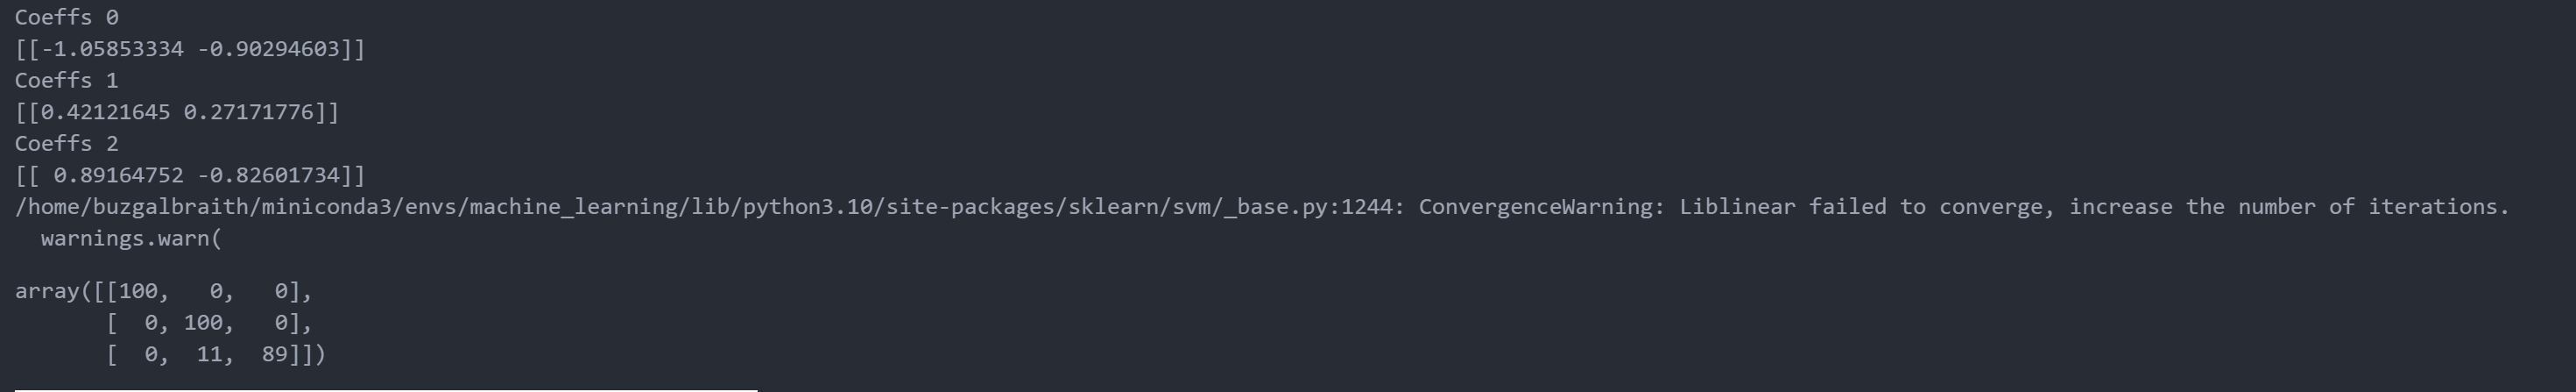
\includegraphics[width=10cm]{homework/homework_5/immages/q1_1.jpg}\item 
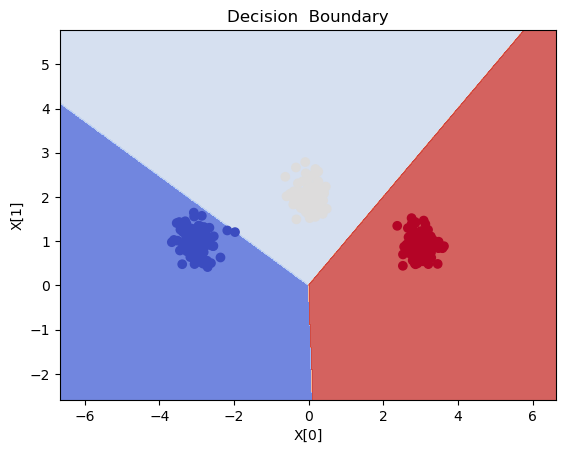
\includegraphics[width=10cm]{homework/homework_5/immages/q1_2.png}
\end{itemize}
\setcounter{saveenum}{\value{enumi}}
\end{enumerate}


\nyuparagraph{Multiclass SVM}

In this question, we will implement stochastic subgradient descent
for the linear multiclass SVM, as described in class and in this
problem set. We will use the class-sensitive feature mapping approach
with the ``multivector construction'', as described in the multiclass lecture.
\begin{enumerate}
  \setcounter{enumi}{\value{saveenum}}
\item Complete the function \texttt{featureMap} in the skeleton code.
\begin{itemize}
    \color{blue}
    \item here i use the np.flatten function 
    \item suppose the output of feature map is in $M\in \mathbb{R}^{n\times d}$. if $n\neq 1$ then squeeze does not effect M, if $n=1$ then squeeze reduces $M$ to the vector $m\in \mathbb{R}^{d}$ which makes dimensions more compatible down the road. 
    \item 
             \inputminted[firstline=132, lastline=144, breaklines=True]{python}{hw_5.py}
\end{itemize}

\item Complete the function \texttt{sgd}.
\begin{itemize}
    \color{blue}
    \item here i used a falling step size because i found it helped convergence 
               \inputminted[firstline=147, lastline=170, breaklines=True]{python}{hw_5.py}
\end{itemize}

\item Complete the methods \texttt{subgradient}, \texttt{decision\_function} and \texttt{predict} from the class \texttt{MulticlassSVM}. 
\begin{itemize}
    \color{blue}
    \item in the subgradient function i check if the max of the hinge loss is 0, because this is equivalent to the true class being in the argmax of the hinge loss, with out needing to rely on the np.argmax() function for discrete class labels.  
               \inputminted[firstline=172, lastline=251, breaklines=True]{python}{hw_5.py}
\end{itemize}

\item Following the multiclass
SVM implementation, we have included another block of test code. Make
sure to include the results from these tests in your assignment, along
with your code. 
\begin{itemize}
    \color{blue}
    \item 

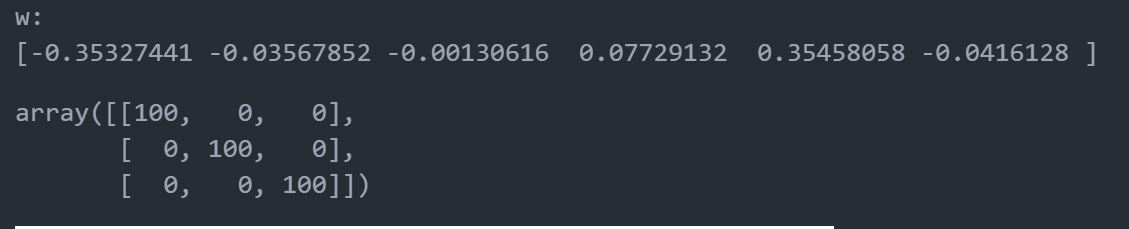
\includegraphics[width=10cm]{homework/homework_5/immages/q2_1.jpg}\item 
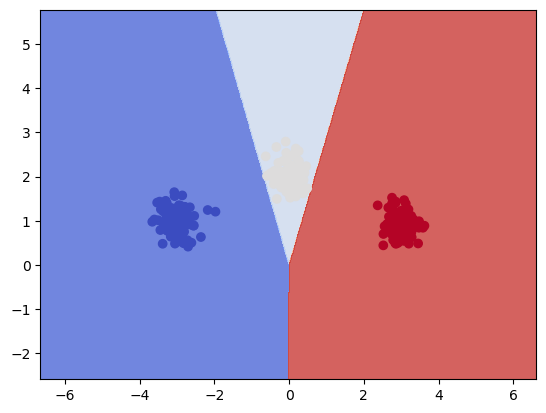
\includegraphics[width=10cm]{homework/homework_5/immages/q2_2.png}
\end{itemize}
\setcounter{saveenum}{\value{enumi}}
\end{enumerate}

\end{document}